\documentclass[twoside]{book}

% Packages required by doxygen
\usepackage{fixltx2e}
\usepackage{calc}
\usepackage{doxygen}
\usepackage[export]{adjustbox} % also loads graphicx
\usepackage{graphicx}
\usepackage[utf8]{inputenc}
\usepackage{makeidx}
\usepackage{multicol}
\usepackage{multirow}
\PassOptionsToPackage{warn}{textcomp}
\usepackage{textcomp}
\usepackage[nointegrals]{wasysym}
\usepackage[table]{xcolor}

% Font selection
\usepackage[T1]{fontenc}
\usepackage[scaled=.90]{helvet}
\usepackage{courier}
\usepackage{amssymb}
\usepackage{sectsty}
\renewcommand{\familydefault}{\sfdefault}
\allsectionsfont{%
  \fontseries{bc}\selectfont%
  \color{darkgray}%
}
\renewcommand{\DoxyLabelFont}{%
  \fontseries{bc}\selectfont%
  \color{darkgray}%
}
\newcommand{\+}{\discretionary{\mbox{\scriptsize$\hookleftarrow$}}{}{}}

% Page & text layout
\usepackage{geometry}
\geometry{%
  a4paper,%
  top=2.5cm,%
  bottom=2.5cm,%
  left=2.5cm,%
  right=2.5cm%
}
\tolerance=750
\hfuzz=15pt
\hbadness=750
\setlength{\emergencystretch}{15pt}
\setlength{\parindent}{0cm}
\setlength{\parskip}{0.2cm}
\makeatletter
\renewcommand{\paragraph}{%
  \@startsection{paragraph}{4}{0ex}{-1.0ex}{1.0ex}{%
    \normalfont\normalsize\bfseries\SS@parafont%
  }%
}
\renewcommand{\subparagraph}{%
  \@startsection{subparagraph}{5}{0ex}{-1.0ex}{1.0ex}{%
    \normalfont\normalsize\bfseries\SS@subparafont%
  }%
}
\makeatother

% Headers & footers
\usepackage{fancyhdr}
\pagestyle{fancyplain}
\fancyhead[LE]{\fancyplain{}{\bfseries\thepage}}
\fancyhead[CE]{\fancyplain{}{}}
\fancyhead[RE]{\fancyplain{}{\bfseries\leftmark}}
\fancyhead[LO]{\fancyplain{}{\bfseries\rightmark}}
\fancyhead[CO]{\fancyplain{}{}}
\fancyhead[RO]{\fancyplain{}{\bfseries\thepage}}
\fancyfoot[LE]{\fancyplain{}{}}
\fancyfoot[CE]{\fancyplain{}{}}
\fancyfoot[RE]{\fancyplain{}{\bfseries\scriptsize Generated on Tue Apr 21 2015 19\+:28\+:21 for Dodger by Doxygen }}
\fancyfoot[LO]{\fancyplain{}{\bfseries\scriptsize Generated on Tue Apr 21 2015 19\+:28\+:21 for Dodger by Doxygen }}
\fancyfoot[CO]{\fancyplain{}{}}
\fancyfoot[RO]{\fancyplain{}{}}
\renewcommand{\footrulewidth}{0.4pt}
\renewcommand{\chaptermark}[1]{%
  \markboth{#1}{}%
}
\renewcommand{\sectionmark}[1]{%
  \markright{\thesection\ #1}%
}

% Indices & bibliography
\usepackage{natbib}
\usepackage[titles]{tocloft}
\setcounter{tocdepth}{3}
\setcounter{secnumdepth}{5}
\makeindex

% Hyperlinks (required, but should be loaded last)
\usepackage{ifpdf}
\ifpdf
  \usepackage[pdftex,pagebackref=true]{hyperref}
\else
  \usepackage[ps2pdf,pagebackref=true]{hyperref}
\fi
\hypersetup{%
  colorlinks=true,%
  linkcolor=blue,%
  citecolor=blue,%
  unicode%
}

% Custom commands
\newcommand{\clearemptydoublepage}{%
  \newpage{\pagestyle{empty}\cleardoublepage}%
}


%===== C O N T E N T S =====

\begin{document}

% Titlepage & ToC
\hypersetup{pageanchor=false,
             bookmarks=true,
             bookmarksnumbered=true,
             pdfencoding=unicode
            }
\pagenumbering{roman}
\begin{titlepage}
\vspace*{7cm}
\begin{center}%
{\Large Dodger }\\
\vspace*{1cm}
{\large Generated by Doxygen 1.8.9.1}\\
\vspace*{0.5cm}
{\small Tue Apr 21 2015 19:28:21}\\
\end{center}
\end{titlepage}
\clearemptydoublepage
\tableofcontents
\clearemptydoublepage
\pagenumbering{arabic}
\hypersetup{pageanchor=true}

%--- Begin generated contents ---
\chapter{Namespace Index}
\section{Namespace List}
Here is a list of all namespaces with brief descriptions\+:\begin{DoxyCompactList}
\item\contentsline{section}{\hyperlink{namespace_dodger}{Dodger} }{\pageref{namespace_dodger}}{}
\item\contentsline{section}{\hyperlink{namespace_dodger_1_1klassid}{Dodger.\+klassid} }{\pageref{namespace_dodger_1_1klassid}}{}
\item\contentsline{section}{\hyperlink{namespace_dodger_1_1main}{Dodger.\+main} }{\pageref{namespace_dodger_1_1main}}{}
\item\contentsline{section}{\hyperlink{namespace_dodger_1_1muutujad}{Dodger.\+muutujad} }{\pageref{namespace_dodger_1_1muutujad}}{}
\end{DoxyCompactList}

\chapter{Hierarchical Index}
\section{Class Hierarchy}
This inheritance list is sorted roughly, but not completely, alphabetically\+:\begin{DoxyCompactList}
\item Sprite\begin{DoxyCompactList}
\item \contentsline{section}{Dodger.\+klassid.\+Mine}{\pageref{class_dodger_1_1klassid_1_1_mine}}{}
\item \contentsline{section}{Dodger.\+klassid.\+Triangle}{\pageref{class_dodger_1_1klassid_1_1_triangle}}{}
\end{DoxyCompactList}
\end{DoxyCompactList}

\chapter{Class Index}
\section{Class List}
Here are the classes, structs, unions and interfaces with brief descriptions\+:\begin{DoxyCompactList}
\item\contentsline{section}{\hyperlink{class_dodger_1_1klassid_1_1_mine}{Dodger.\+klassid.\+Mine} }{\pageref{class_dodger_1_1klassid_1_1_mine}}{}
\item\contentsline{section}{\hyperlink{class_dodger_1_1klassid_1_1_triangle}{Dodger.\+klassid.\+Triangle} }{\pageref{class_dodger_1_1klassid_1_1_triangle}}{}
\end{DoxyCompactList}

\chapter{File Index}
\section{File List}
Here is a list of all files with brief descriptions\+:\begin{DoxyCompactList}
\item\contentsline{section}{\hyperlink{____init_____8py}{\+\_\+\+\_\+init\+\_\+\+\_\+.\+py} }{\pageref{____init_____8py}}{}
\item\contentsline{section}{\hyperlink{klassid_8py}{klassid.\+py} }{\pageref{klassid_8py}}{}
\item\contentsline{section}{\hyperlink{main_8py}{main.\+py} }{\pageref{main_8py}}{}
\item\contentsline{section}{\hyperlink{muutujad_8py}{muutujad.\+py} }{\pageref{muutujad_8py}}{}
\end{DoxyCompactList}

\chapter{Namespace Documentation}
\hypertarget{namespace_dodger}{}\section{Dodger Namespace Reference}
\label{namespace_dodger}\index{Dodger@{Dodger}}
\subsection*{Namespaces}
\begin{DoxyCompactItemize}
\item 
 \hyperlink{namespace_dodger_1_1klassid}{klassid}
\item 
 \hyperlink{namespace_dodger_1_1main}{main}
\item 
 \hyperlink{namespace_dodger_1_1muutujad}{muutujad}
\end{DoxyCompactItemize}

\hypertarget{namespace_dodger_1_1klassid}{}\section{Dodger.\+klassid Namespace Reference}
\label{namespace_dodger_1_1klassid}\index{Dodger.\+klassid@{Dodger.\+klassid}}
\subsection*{Classes}
\begin{DoxyCompactItemize}
\item 
class \hyperlink{class_dodger_1_1klassid_1_1_mine}{Mine}
\item 
class \hyperlink{class_dodger_1_1klassid_1_1_triangle}{Triangle}
\end{DoxyCompactItemize}

\hypertarget{namespace_dodger_1_1main}{}\section{Dodger.\+main Namespace Reference}
\label{namespace_dodger_1_1main}\index{Dodger.\+main@{Dodger.\+main}}
\subsection*{Functions}
\begin{DoxyCompactItemize}
\item 
def \hyperlink{namespace_dodger_1_1main_a4c06079e7a33bf58a26e3bcab04c612d}{reset} ()
\item 
def \hyperlink{namespace_dodger_1_1main_ad002f84c7d1646af7ac367a665eec672}{skoor} (score)
\end{DoxyCompactItemize}
\subsection*{Variables}
\begin{DoxyCompactItemize}
\item 
tuple \hyperlink{namespace_dodger_1_1main_a5a2e204b9d9a091c33208dd3657e1307}{myfont} = pygame.\+font.\+Sys\+Font(\char`\"{}monospace\char`\"{}, 15)
\item 
tuple \hyperlink{namespace_dodger_1_1main_aae789c71f775508744848c9b4163b416}{screen} = pygame.\+display.\+set\+\_\+mode(\mbox{[}800,600\mbox{]})
\item 
tuple \hyperlink{namespace_dodger_1_1main_a688c4b7dc0b19589a3f62d27a0233a7f}{clock} = pygame.\+time.\+Clock()
\item 
tuple \hyperlink{namespace_dodger_1_1main_aada8d7b289e64fa2cd4da076de1f23c2}{tervist} = myfont.\+render(\char`\"{}Press S\+P\+A\+C\+E to begin.\char`\"{}, 10, muutujad.\+green)
\item 
tuple \hyperlink{namespace_dodger_1_1main_ab3023da733d7bcce7908efc9e646a3d1}{tervist1} = myfont.\+render(\char`\"{}Press R to reset.\char`\"{}, 10, muutujad.\+green)
\item 
tuple \hyperlink{namespace_dodger_1_1main_abc3f766e093308afeae4bb11717428ee}{kinni} = myfont.\+render(\char`\"{}Press S\+P\+A\+C\+E to exit.\char`\"{}, 10, muutujad.\+green)
\item 
tuple \hyperlink{namespace_dodger_1_1main_a4794605b0906db6c42412957da8c5913}{triangle\+\_\+sprite} = pygame.\+sprite.\+Group()
\item 
tuple \hyperlink{namespace_dodger_1_1main_a8ef3adbca26416fcae28a066e6435001}{all\+\_\+sprites} = pygame.\+sprite.\+Group()
\item 
tuple \hyperlink{namespace_dodger_1_1main_a9ce66d4a60e19c14f89b870a580099e4}{mine} = \hyperlink{class_dodger_1_1klassid_1_1_mine}{klassid.\+Mine}(random.\+randrange(0, 800),random.\+randrange(0, 100))
\item 
tuple \hyperlink{namespace_dodger_1_1main_ab1f09b41f09bcf1417ed69012e847012}{alfa\+\_\+mine} = \hyperlink{class_dodger_1_1klassid_1_1_mine}{klassid.\+Mine}(-\/100,random.\+randrange(0, 100))
\item 
tuple \hyperlink{namespace_dodger_1_1main_a5c27661b1b9c13624a07f3757a3bd88a}{triangle} = \hyperlink{class_dodger_1_1klassid_1_1_triangle}{klassid.\+Triangle}(400, 555)
\item 
\hyperlink{namespace_dodger_1_1main_a53770c6e2fd58e07592f4ac4dca29689}{beginning} = True
\item 
\hyperlink{namespace_dodger_1_1main_a2c62876655c9247b65a382ebe35239a8}{running} = False
\item 
\hyperlink{namespace_dodger_1_1main_a13868600ce1e836d5d3e848a5932231d}{over} = False
\item 
tuple \hyperlink{namespace_dodger_1_1main_a6c470cdcf880300fb28ae58cf38bfb92}{lose} = myfont.\+render(\char`\"{}Game over!\char`\"{}, 1, muutujad.\+green)
\end{DoxyCompactItemize}


\subsection{Function Documentation}
\hypertarget{namespace_dodger_1_1main_a4c06079e7a33bf58a26e3bcab04c612d}{}\index{Dodger\+::main@{Dodger\+::main}!reset@{reset}}
\index{reset@{reset}!Dodger\+::main@{Dodger\+::main}}
\subsubsection[{reset}]{\setlength{\rightskip}{0pt plus 5cm}def Dodger.\+main.\+reset (
\begin{DoxyParamCaption}
{}
\end{DoxyParamCaption}
)}\label{namespace_dodger_1_1main_a4c06079e7a33bf58a26e3bcab04c612d}
\hypertarget{namespace_dodger_1_1main_ad002f84c7d1646af7ac367a665eec672}{}\index{Dodger\+::main@{Dodger\+::main}!skoor@{skoor}}
\index{skoor@{skoor}!Dodger\+::main@{Dodger\+::main}}
\subsubsection[{skoor}]{\setlength{\rightskip}{0pt plus 5cm}def Dodger.\+main.\+skoor (
\begin{DoxyParamCaption}
\item[{}]{score}
\end{DoxyParamCaption}
)}\label{namespace_dodger_1_1main_ad002f84c7d1646af7ac367a665eec672}


\subsection{Variable Documentation}
\hypertarget{namespace_dodger_1_1main_ab1f09b41f09bcf1417ed69012e847012}{}\index{Dodger\+::main@{Dodger\+::main}!alfa\+\_\+mine@{alfa\+\_\+mine}}
\index{alfa\+\_\+mine@{alfa\+\_\+mine}!Dodger\+::main@{Dodger\+::main}}
\subsubsection[{alfa\+\_\+mine}]{\setlength{\rightskip}{0pt plus 5cm}tuple Dodger.\+main.\+alfa\+\_\+mine = {\bf klassid.\+Mine}(-\/100,random.\+randrange(0, 100))}\label{namespace_dodger_1_1main_ab1f09b41f09bcf1417ed69012e847012}
\hypertarget{namespace_dodger_1_1main_a8ef3adbca26416fcae28a066e6435001}{}\index{Dodger\+::main@{Dodger\+::main}!all\+\_\+sprites@{all\+\_\+sprites}}
\index{all\+\_\+sprites@{all\+\_\+sprites}!Dodger\+::main@{Dodger\+::main}}
\subsubsection[{all\+\_\+sprites}]{\setlength{\rightskip}{0pt plus 5cm}tuple Dodger.\+main.\+all\+\_\+sprites = pygame.\+sprite.\+Group()}\label{namespace_dodger_1_1main_a8ef3adbca26416fcae28a066e6435001}
\hypertarget{namespace_dodger_1_1main_a53770c6e2fd58e07592f4ac4dca29689}{}\index{Dodger\+::main@{Dodger\+::main}!beginning@{beginning}}
\index{beginning@{beginning}!Dodger\+::main@{Dodger\+::main}}
\subsubsection[{beginning}]{\setlength{\rightskip}{0pt plus 5cm}Dodger.\+main.\+beginning = True}\label{namespace_dodger_1_1main_a53770c6e2fd58e07592f4ac4dca29689}
\hypertarget{namespace_dodger_1_1main_a688c4b7dc0b19589a3f62d27a0233a7f}{}\index{Dodger\+::main@{Dodger\+::main}!clock@{clock}}
\index{clock@{clock}!Dodger\+::main@{Dodger\+::main}}
\subsubsection[{clock}]{\setlength{\rightskip}{0pt plus 5cm}tuple Dodger.\+main.\+clock = pygame.\+time.\+Clock()}\label{namespace_dodger_1_1main_a688c4b7dc0b19589a3f62d27a0233a7f}
\hypertarget{namespace_dodger_1_1main_abc3f766e093308afeae4bb11717428ee}{}\index{Dodger\+::main@{Dodger\+::main}!kinni@{kinni}}
\index{kinni@{kinni}!Dodger\+::main@{Dodger\+::main}}
\subsubsection[{kinni}]{\setlength{\rightskip}{0pt plus 5cm}tuple Dodger.\+main.\+kinni = myfont.\+render(\char`\"{}Press S\+P\+A\+C\+E to exit.\char`\"{}, 10, muutujad.\+green)}\label{namespace_dodger_1_1main_abc3f766e093308afeae4bb11717428ee}
\hypertarget{namespace_dodger_1_1main_a6c470cdcf880300fb28ae58cf38bfb92}{}\index{Dodger\+::main@{Dodger\+::main}!lose@{lose}}
\index{lose@{lose}!Dodger\+::main@{Dodger\+::main}}
\subsubsection[{lose}]{\setlength{\rightskip}{0pt plus 5cm}tuple Dodger.\+main.\+lose = myfont.\+render(\char`\"{}Game over!\char`\"{}, 1, muutujad.\+green)}\label{namespace_dodger_1_1main_a6c470cdcf880300fb28ae58cf38bfb92}
\hypertarget{namespace_dodger_1_1main_a9ce66d4a60e19c14f89b870a580099e4}{}\index{Dodger\+::main@{Dodger\+::main}!mine@{mine}}
\index{mine@{mine}!Dodger\+::main@{Dodger\+::main}}
\subsubsection[{mine}]{\setlength{\rightskip}{0pt plus 5cm}tuple Dodger.\+main.\+mine = {\bf klassid.\+Mine}(random.\+randrange(0, 800),random.\+randrange(0, 100))}\label{namespace_dodger_1_1main_a9ce66d4a60e19c14f89b870a580099e4}
\hypertarget{namespace_dodger_1_1main_a5a2e204b9d9a091c33208dd3657e1307}{}\index{Dodger\+::main@{Dodger\+::main}!myfont@{myfont}}
\index{myfont@{myfont}!Dodger\+::main@{Dodger\+::main}}
\subsubsection[{myfont}]{\setlength{\rightskip}{0pt plus 5cm}tuple Dodger.\+main.\+myfont = pygame.\+font.\+Sys\+Font(\char`\"{}monospace\char`\"{}, 15)}\label{namespace_dodger_1_1main_a5a2e204b9d9a091c33208dd3657e1307}
\hypertarget{namespace_dodger_1_1main_a13868600ce1e836d5d3e848a5932231d}{}\index{Dodger\+::main@{Dodger\+::main}!over@{over}}
\index{over@{over}!Dodger\+::main@{Dodger\+::main}}
\subsubsection[{over}]{\setlength{\rightskip}{0pt plus 5cm}Dodger.\+main.\+over = False}\label{namespace_dodger_1_1main_a13868600ce1e836d5d3e848a5932231d}
\hypertarget{namespace_dodger_1_1main_a2c62876655c9247b65a382ebe35239a8}{}\index{Dodger\+::main@{Dodger\+::main}!running@{running}}
\index{running@{running}!Dodger\+::main@{Dodger\+::main}}
\subsubsection[{running}]{\setlength{\rightskip}{0pt plus 5cm}Dodger.\+main.\+running = False}\label{namespace_dodger_1_1main_a2c62876655c9247b65a382ebe35239a8}
\hypertarget{namespace_dodger_1_1main_aae789c71f775508744848c9b4163b416}{}\index{Dodger\+::main@{Dodger\+::main}!screen@{screen}}
\index{screen@{screen}!Dodger\+::main@{Dodger\+::main}}
\subsubsection[{screen}]{\setlength{\rightskip}{0pt plus 5cm}tuple Dodger.\+main.\+screen = pygame.\+display.\+set\+\_\+mode(\mbox{[}800,600\mbox{]})}\label{namespace_dodger_1_1main_aae789c71f775508744848c9b4163b416}
\hypertarget{namespace_dodger_1_1main_aada8d7b289e64fa2cd4da076de1f23c2}{}\index{Dodger\+::main@{Dodger\+::main}!tervist@{tervist}}
\index{tervist@{tervist}!Dodger\+::main@{Dodger\+::main}}
\subsubsection[{tervist}]{\setlength{\rightskip}{0pt plus 5cm}tuple Dodger.\+main.\+tervist = myfont.\+render(\char`\"{}Press S\+P\+A\+C\+E to begin.\char`\"{}, 10, muutujad.\+green)}\label{namespace_dodger_1_1main_aada8d7b289e64fa2cd4da076de1f23c2}
\hypertarget{namespace_dodger_1_1main_ab3023da733d7bcce7908efc9e646a3d1}{}\index{Dodger\+::main@{Dodger\+::main}!tervist1@{tervist1}}
\index{tervist1@{tervist1}!Dodger\+::main@{Dodger\+::main}}
\subsubsection[{tervist1}]{\setlength{\rightskip}{0pt plus 5cm}tuple Dodger.\+main.\+tervist1 = myfont.\+render(\char`\"{}Press R to reset.\char`\"{}, 10, muutujad.\+green)}\label{namespace_dodger_1_1main_ab3023da733d7bcce7908efc9e646a3d1}
\hypertarget{namespace_dodger_1_1main_a5c27661b1b9c13624a07f3757a3bd88a}{}\index{Dodger\+::main@{Dodger\+::main}!triangle@{triangle}}
\index{triangle@{triangle}!Dodger\+::main@{Dodger\+::main}}
\subsubsection[{triangle}]{\setlength{\rightskip}{0pt plus 5cm}tuple Dodger.\+main.\+triangle = {\bf klassid.\+Triangle}(400, 555)}\label{namespace_dodger_1_1main_a5c27661b1b9c13624a07f3757a3bd88a}
\hypertarget{namespace_dodger_1_1main_a4794605b0906db6c42412957da8c5913}{}\index{Dodger\+::main@{Dodger\+::main}!triangle\+\_\+sprite@{triangle\+\_\+sprite}}
\index{triangle\+\_\+sprite@{triangle\+\_\+sprite}!Dodger\+::main@{Dodger\+::main}}
\subsubsection[{triangle\+\_\+sprite}]{\setlength{\rightskip}{0pt plus 5cm}tuple Dodger.\+main.\+triangle\+\_\+sprite = pygame.\+sprite.\+Group()}\label{namespace_dodger_1_1main_a4794605b0906db6c42412957da8c5913}

\hypertarget{namespace_dodger_1_1muutujad}{}\section{Dodger.\+muutujad Namespace Reference}
\label{namespace_dodger_1_1muutujad}\index{Dodger.\+muutujad@{Dodger.\+muutujad}}
\subsection*{Variables}
\begin{DoxyCompactItemize}
\item 
list \hyperlink{namespace_dodger_1_1muutujad_a950ccd86c2731c52ece948ce302c6f96}{white} = \mbox{[}255,255,255\mbox{]}
\item 
list \hyperlink{namespace_dodger_1_1muutujad_a443de8a68ebc1f25f1595be74116ba7c}{black} = \mbox{[}0,0,0\mbox{]}
\item 
list \hyperlink{namespace_dodger_1_1muutujad_a9a3c4c00825bcf1180f94222380aef68}{green} = \mbox{[}0,255,0\mbox{]}
\item 
int \hyperlink{namespace_dodger_1_1muutujad_ae7c3ed6b4ef11513d11310b665039cd1}{samm} = 5
\item 
int \hyperlink{namespace_dodger_1_1muutujad_a9607e1aed5a091af3b0c14ec1beab289}{score} = 0
\item 
int \hyperlink{namespace_dodger_1_1muutujad_ad597bc6d76e9941c159e6ea9fb6695ba}{kordus} = 0
\end{DoxyCompactItemize}


\subsection{Variable Documentation}
\hypertarget{namespace_dodger_1_1muutujad_a443de8a68ebc1f25f1595be74116ba7c}{}\index{Dodger\+::muutujad@{Dodger\+::muutujad}!black@{black}}
\index{black@{black}!Dodger\+::muutujad@{Dodger\+::muutujad}}
\subsubsection[{black}]{\setlength{\rightskip}{0pt plus 5cm}list Dodger.\+muutujad.\+black = \mbox{[}0,0,0\mbox{]}}\label{namespace_dodger_1_1muutujad_a443de8a68ebc1f25f1595be74116ba7c}
\hypertarget{namespace_dodger_1_1muutujad_a9a3c4c00825bcf1180f94222380aef68}{}\index{Dodger\+::muutujad@{Dodger\+::muutujad}!green@{green}}
\index{green@{green}!Dodger\+::muutujad@{Dodger\+::muutujad}}
\subsubsection[{green}]{\setlength{\rightskip}{0pt plus 5cm}list Dodger.\+muutujad.\+green = \mbox{[}0,255,0\mbox{]}}\label{namespace_dodger_1_1muutujad_a9a3c4c00825bcf1180f94222380aef68}
\hypertarget{namespace_dodger_1_1muutujad_ad597bc6d76e9941c159e6ea9fb6695ba}{}\index{Dodger\+::muutujad@{Dodger\+::muutujad}!kordus@{kordus}}
\index{kordus@{kordus}!Dodger\+::muutujad@{Dodger\+::muutujad}}
\subsubsection[{kordus}]{\setlength{\rightskip}{0pt plus 5cm}int Dodger.\+muutujad.\+kordus = 0}\label{namespace_dodger_1_1muutujad_ad597bc6d76e9941c159e6ea9fb6695ba}
\hypertarget{namespace_dodger_1_1muutujad_ae7c3ed6b4ef11513d11310b665039cd1}{}\index{Dodger\+::muutujad@{Dodger\+::muutujad}!samm@{samm}}
\index{samm@{samm}!Dodger\+::muutujad@{Dodger\+::muutujad}}
\subsubsection[{samm}]{\setlength{\rightskip}{0pt plus 5cm}int Dodger.\+muutujad.\+samm = 5}\label{namespace_dodger_1_1muutujad_ae7c3ed6b4ef11513d11310b665039cd1}
\hypertarget{namespace_dodger_1_1muutujad_a9607e1aed5a091af3b0c14ec1beab289}{}\index{Dodger\+::muutujad@{Dodger\+::muutujad}!score@{score}}
\index{score@{score}!Dodger\+::muutujad@{Dodger\+::muutujad}}
\subsubsection[{score}]{\setlength{\rightskip}{0pt plus 5cm}int Dodger.\+muutujad.\+score = 0}\label{namespace_dodger_1_1muutujad_a9607e1aed5a091af3b0c14ec1beab289}
\hypertarget{namespace_dodger_1_1muutujad_a950ccd86c2731c52ece948ce302c6f96}{}\index{Dodger\+::muutujad@{Dodger\+::muutujad}!white@{white}}
\index{white@{white}!Dodger\+::muutujad@{Dodger\+::muutujad}}
\subsubsection[{white}]{\setlength{\rightskip}{0pt plus 5cm}list Dodger.\+muutujad.\+white = \mbox{[}255,255,255\mbox{]}}\label{namespace_dodger_1_1muutujad_a950ccd86c2731c52ece948ce302c6f96}

\chapter{Class Documentation}
\hypertarget{class_dodger_1_1klassid_1_1_mine}{}\section{Dodger.\+klassid.\+Mine Class Reference}
\label{class_dodger_1_1klassid_1_1_mine}\index{Dodger.\+klassid.\+Mine@{Dodger.\+klassid.\+Mine}}
Inheritance diagram for Dodger.\+klassid.\+Mine\+:\begin{figure}[H]
\begin{center}
\leavevmode
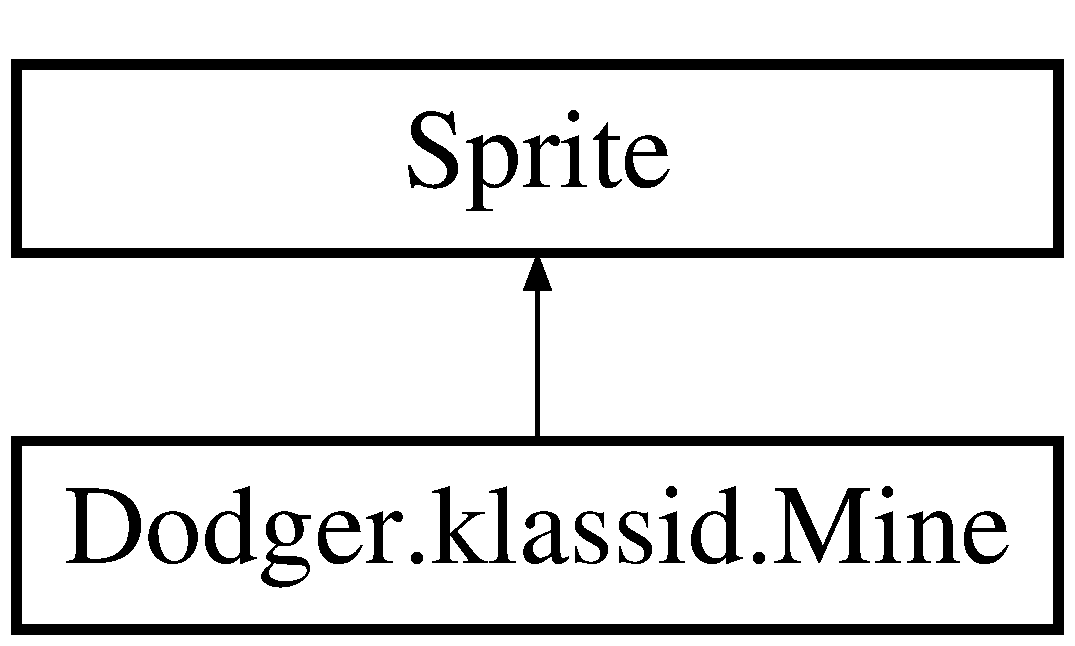
\includegraphics[height=2.000000cm]{class_dodger_1_1klassid_1_1_mine}
\end{center}
\end{figure}
\subsection*{Public Member Functions}
\begin{DoxyCompactItemize}
\item 
def \hyperlink{class_dodger_1_1klassid_1_1_mine_a0dc99bc7580ee7a9bd155dec1b66df98}{\+\_\+\+\_\+init\+\_\+\+\_\+} (self, \hyperlink{class_dodger_1_1klassid_1_1_mine_accdd2e2ec2e81511337e183369d5916a}{x}, \hyperlink{class_dodger_1_1klassid_1_1_mine_a634b0ff493f5bba0350fc58d09eb040d}{y})
\item 
def \hyperlink{class_dodger_1_1klassid_1_1_mine_aec34add3ad847964539079cbb200e79a}{reset\+\_\+pos} (self)
\item 
def \hyperlink{class_dodger_1_1klassid_1_1_mine_a8854f857140ecccdd9251c86605aaf79}{update} (self, pikkus, kordus)
\end{DoxyCompactItemize}
\subsection*{Public Attributes}
\begin{DoxyCompactItemize}
\item 
\hyperlink{class_dodger_1_1klassid_1_1_mine_accdd2e2ec2e81511337e183369d5916a}{x}
\item 
\hyperlink{class_dodger_1_1klassid_1_1_mine_a634b0ff493f5bba0350fc58d09eb040d}{y}
\item 
\hyperlink{class_dodger_1_1klassid_1_1_mine_a95e8cfdeb751fc7180cec6eeb8bb337b}{image}
\item 
\hyperlink{class_dodger_1_1klassid_1_1_mine_a268ed423734c64d9b2b2bc36012d134f}{rect}
\end{DoxyCompactItemize}


\subsection{Detailed Description}
\begin{DoxyVerb}Miinide klass, mis kontrollib miinide tegevust.
\end{DoxyVerb}
 

\subsection{Constructor \& Destructor Documentation}
\hypertarget{class_dodger_1_1klassid_1_1_mine_a0dc99bc7580ee7a9bd155dec1b66df98}{}\index{Dodger\+::klassid\+::\+Mine@{Dodger\+::klassid\+::\+Mine}!\+\_\+\+\_\+init\+\_\+\+\_\+@{\+\_\+\+\_\+init\+\_\+\+\_\+}}
\index{\+\_\+\+\_\+init\+\_\+\+\_\+@{\+\_\+\+\_\+init\+\_\+\+\_\+}!Dodger\+::klassid\+::\+Mine@{Dodger\+::klassid\+::\+Mine}}
\subsubsection[{\+\_\+\+\_\+init\+\_\+\+\_\+}]{\setlength{\rightskip}{0pt plus 5cm}def Dodger.\+klassid.\+Mine.\+\_\+\+\_\+init\+\_\+\+\_\+ (
\begin{DoxyParamCaption}
\item[{}]{self, }
\item[{}]{x, }
\item[{}]{y}
\end{DoxyParamCaption}
)}\label{class_dodger_1_1klassid_1_1_mine_a0dc99bc7580ee7a9bd155dec1b66df98}


\subsection{Member Function Documentation}
\hypertarget{class_dodger_1_1klassid_1_1_mine_aec34add3ad847964539079cbb200e79a}{}\index{Dodger\+::klassid\+::\+Mine@{Dodger\+::klassid\+::\+Mine}!reset\+\_\+pos@{reset\+\_\+pos}}
\index{reset\+\_\+pos@{reset\+\_\+pos}!Dodger\+::klassid\+::\+Mine@{Dodger\+::klassid\+::\+Mine}}
\subsubsection[{reset\+\_\+pos}]{\setlength{\rightskip}{0pt plus 5cm}def Dodger.\+klassid.\+Mine.\+reset\+\_\+pos (
\begin{DoxyParamCaption}
\item[{}]{self}
\end{DoxyParamCaption}
)}\label{class_dodger_1_1klassid_1_1_mine_aec34add3ad847964539079cbb200e79a}
\hypertarget{class_dodger_1_1klassid_1_1_mine_a8854f857140ecccdd9251c86605aaf79}{}\index{Dodger\+::klassid\+::\+Mine@{Dodger\+::klassid\+::\+Mine}!update@{update}}
\index{update@{update}!Dodger\+::klassid\+::\+Mine@{Dodger\+::klassid\+::\+Mine}}
\subsubsection[{update}]{\setlength{\rightskip}{0pt plus 5cm}def Dodger.\+klassid.\+Mine.\+update (
\begin{DoxyParamCaption}
\item[{}]{self, }
\item[{}]{pikkus, }
\item[{}]{kordus}
\end{DoxyParamCaption}
)}\label{class_dodger_1_1klassid_1_1_mine_a8854f857140ecccdd9251c86605aaf79}


\subsection{Member Data Documentation}
\hypertarget{class_dodger_1_1klassid_1_1_mine_a95e8cfdeb751fc7180cec6eeb8bb337b}{}\index{Dodger\+::klassid\+::\+Mine@{Dodger\+::klassid\+::\+Mine}!image@{image}}
\index{image@{image}!Dodger\+::klassid\+::\+Mine@{Dodger\+::klassid\+::\+Mine}}
\subsubsection[{image}]{\setlength{\rightskip}{0pt plus 5cm}Dodger.\+klassid.\+Mine.\+image}\label{class_dodger_1_1klassid_1_1_mine_a95e8cfdeb751fc7180cec6eeb8bb337b}
\hypertarget{class_dodger_1_1klassid_1_1_mine_a268ed423734c64d9b2b2bc36012d134f}{}\index{Dodger\+::klassid\+::\+Mine@{Dodger\+::klassid\+::\+Mine}!rect@{rect}}
\index{rect@{rect}!Dodger\+::klassid\+::\+Mine@{Dodger\+::klassid\+::\+Mine}}
\subsubsection[{rect}]{\setlength{\rightskip}{0pt plus 5cm}Dodger.\+klassid.\+Mine.\+rect}\label{class_dodger_1_1klassid_1_1_mine_a268ed423734c64d9b2b2bc36012d134f}
\hypertarget{class_dodger_1_1klassid_1_1_mine_accdd2e2ec2e81511337e183369d5916a}{}\index{Dodger\+::klassid\+::\+Mine@{Dodger\+::klassid\+::\+Mine}!x@{x}}
\index{x@{x}!Dodger\+::klassid\+::\+Mine@{Dodger\+::klassid\+::\+Mine}}
\subsubsection[{x}]{\setlength{\rightskip}{0pt plus 5cm}Dodger.\+klassid.\+Mine.\+x}\label{class_dodger_1_1klassid_1_1_mine_accdd2e2ec2e81511337e183369d5916a}
\hypertarget{class_dodger_1_1klassid_1_1_mine_a634b0ff493f5bba0350fc58d09eb040d}{}\index{Dodger\+::klassid\+::\+Mine@{Dodger\+::klassid\+::\+Mine}!y@{y}}
\index{y@{y}!Dodger\+::klassid\+::\+Mine@{Dodger\+::klassid\+::\+Mine}}
\subsubsection[{y}]{\setlength{\rightskip}{0pt plus 5cm}Dodger.\+klassid.\+Mine.\+y}\label{class_dodger_1_1klassid_1_1_mine_a634b0ff493f5bba0350fc58d09eb040d}


The documentation for this class was generated from the following file\+:\begin{DoxyCompactItemize}
\item 
\hyperlink{klassid_8py}{klassid.\+py}\end{DoxyCompactItemize}

\hypertarget{class_dodger_1_1klassid_1_1_triangle}{}\section{Dodger.\+klassid.\+Triangle Class Reference}
\label{class_dodger_1_1klassid_1_1_triangle}\index{Dodger.\+klassid.\+Triangle@{Dodger.\+klassid.\+Triangle}}
Inheritance diagram for Dodger.\+klassid.\+Triangle\+:\begin{figure}[H]
\begin{center}
\leavevmode
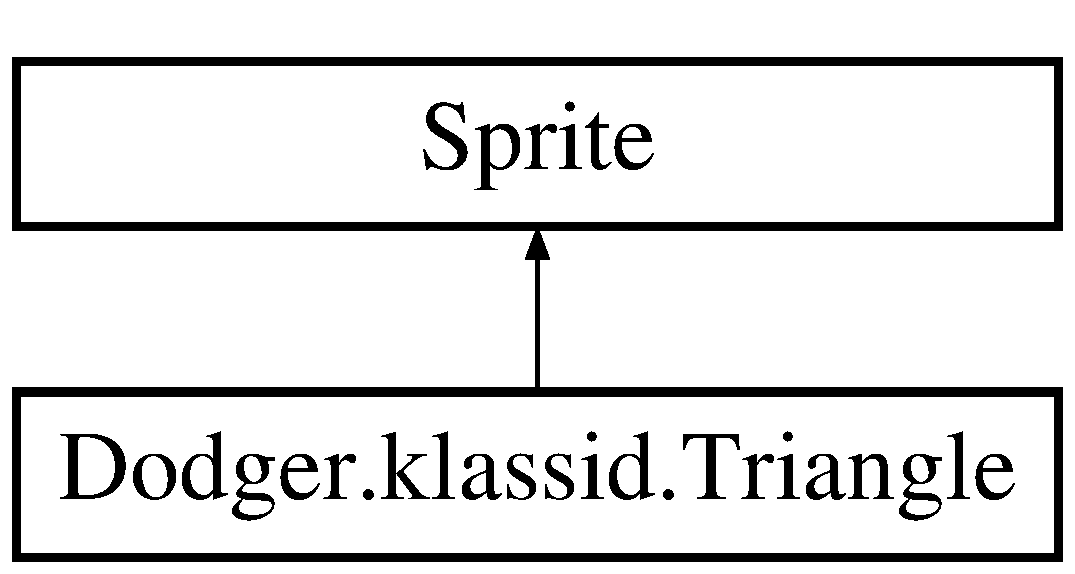
\includegraphics[height=2.000000cm]{class_dodger_1_1klassid_1_1_triangle}
\end{center}
\end{figure}
\subsection*{Public Member Functions}
\begin{DoxyCompactItemize}
\item 
def \hyperlink{class_dodger_1_1klassid_1_1_triangle_a7eaf0a102d5a2ad5e549b73842cd8854}{\+\_\+\+\_\+init\+\_\+\+\_\+} (self, \hyperlink{class_dodger_1_1klassid_1_1_triangle_a17a330d3cf14156818f35ca702d11bee}{x}, \hyperlink{class_dodger_1_1klassid_1_1_triangle_a36eb6984b804d8702084420f442d7917}{y})
\end{DoxyCompactItemize}
\subsection*{Public Attributes}
\begin{DoxyCompactItemize}
\item 
\hyperlink{class_dodger_1_1klassid_1_1_triangle_a17a330d3cf14156818f35ca702d11bee}{x}
\item 
\hyperlink{class_dodger_1_1klassid_1_1_triangle_a36eb6984b804d8702084420f442d7917}{y}
\item 
\hyperlink{class_dodger_1_1klassid_1_1_triangle_a9b7fe7062ff2875d4de3221a3c2e4713}{image}
\item 
\hyperlink{class_dodger_1_1klassid_1_1_triangle_a050d0b0e4a98555475e3f4fc2ab7b863}{rect}
\end{DoxyCompactItemize}


\subsection{Detailed Description}
\begin{DoxyVerb}Playeri klass. Selle abil tehakse sprite, mida saab nooltega juhtida.
\end{DoxyVerb}
 

\subsection{Constructor \& Destructor Documentation}
\hypertarget{class_dodger_1_1klassid_1_1_triangle_a7eaf0a102d5a2ad5e549b73842cd8854}{}\index{Dodger\+::klassid\+::\+Triangle@{Dodger\+::klassid\+::\+Triangle}!\+\_\+\+\_\+init\+\_\+\+\_\+@{\+\_\+\+\_\+init\+\_\+\+\_\+}}
\index{\+\_\+\+\_\+init\+\_\+\+\_\+@{\+\_\+\+\_\+init\+\_\+\+\_\+}!Dodger\+::klassid\+::\+Triangle@{Dodger\+::klassid\+::\+Triangle}}
\subsubsection[{\+\_\+\+\_\+init\+\_\+\+\_\+}]{\setlength{\rightskip}{0pt plus 5cm}def Dodger.\+klassid.\+Triangle.\+\_\+\+\_\+init\+\_\+\+\_\+ (
\begin{DoxyParamCaption}
\item[{}]{self, }
\item[{}]{x, }
\item[{}]{y}
\end{DoxyParamCaption}
)}\label{class_dodger_1_1klassid_1_1_triangle_a7eaf0a102d5a2ad5e549b73842cd8854}


\subsection{Member Data Documentation}
\hypertarget{class_dodger_1_1klassid_1_1_triangle_a9b7fe7062ff2875d4de3221a3c2e4713}{}\index{Dodger\+::klassid\+::\+Triangle@{Dodger\+::klassid\+::\+Triangle}!image@{image}}
\index{image@{image}!Dodger\+::klassid\+::\+Triangle@{Dodger\+::klassid\+::\+Triangle}}
\subsubsection[{image}]{\setlength{\rightskip}{0pt plus 5cm}Dodger.\+klassid.\+Triangle.\+image}\label{class_dodger_1_1klassid_1_1_triangle_a9b7fe7062ff2875d4de3221a3c2e4713}
\hypertarget{class_dodger_1_1klassid_1_1_triangle_a050d0b0e4a98555475e3f4fc2ab7b863}{}\index{Dodger\+::klassid\+::\+Triangle@{Dodger\+::klassid\+::\+Triangle}!rect@{rect}}
\index{rect@{rect}!Dodger\+::klassid\+::\+Triangle@{Dodger\+::klassid\+::\+Triangle}}
\subsubsection[{rect}]{\setlength{\rightskip}{0pt plus 5cm}Dodger.\+klassid.\+Triangle.\+rect}\label{class_dodger_1_1klassid_1_1_triangle_a050d0b0e4a98555475e3f4fc2ab7b863}
\hypertarget{class_dodger_1_1klassid_1_1_triangle_a17a330d3cf14156818f35ca702d11bee}{}\index{Dodger\+::klassid\+::\+Triangle@{Dodger\+::klassid\+::\+Triangle}!x@{x}}
\index{x@{x}!Dodger\+::klassid\+::\+Triangle@{Dodger\+::klassid\+::\+Triangle}}
\subsubsection[{x}]{\setlength{\rightskip}{0pt plus 5cm}Dodger.\+klassid.\+Triangle.\+x}\label{class_dodger_1_1klassid_1_1_triangle_a17a330d3cf14156818f35ca702d11bee}
\hypertarget{class_dodger_1_1klassid_1_1_triangle_a36eb6984b804d8702084420f442d7917}{}\index{Dodger\+::klassid\+::\+Triangle@{Dodger\+::klassid\+::\+Triangle}!y@{y}}
\index{y@{y}!Dodger\+::klassid\+::\+Triangle@{Dodger\+::klassid\+::\+Triangle}}
\subsubsection[{y}]{\setlength{\rightskip}{0pt plus 5cm}Dodger.\+klassid.\+Triangle.\+y}\label{class_dodger_1_1klassid_1_1_triangle_a36eb6984b804d8702084420f442d7917}


The documentation for this class was generated from the following file\+:\begin{DoxyCompactItemize}
\item 
\hyperlink{klassid_8py}{klassid.\+py}\end{DoxyCompactItemize}

\chapter{File Documentation}
\hypertarget{____init_____8py}{}\section{\+\_\+\+\_\+init\+\_\+\+\_\+.\+py File Reference}
\label{____init_____8py}\index{\+\_\+\+\_\+init\+\_\+\+\_\+.\+py@{\+\_\+\+\_\+init\+\_\+\+\_\+.\+py}}
\subsection*{Namespaces}
\begin{DoxyCompactItemize}
\item 
 \hyperlink{namespace_dodger}{Dodger}
\end{DoxyCompactItemize}

\hypertarget{klassid_8py}{}\section{klassid.\+py File Reference}
\label{klassid_8py}\index{klassid.\+py@{klassid.\+py}}
\subsection*{Classes}
\begin{DoxyCompactItemize}
\item 
class \hyperlink{class_dodger_1_1klassid_1_1_triangle}{Dodger.\+klassid.\+Triangle}
\item 
class \hyperlink{class_dodger_1_1klassid_1_1_mine}{Dodger.\+klassid.\+Mine}
\end{DoxyCompactItemize}
\subsection*{Namespaces}
\begin{DoxyCompactItemize}
\item 
 \hyperlink{namespace_dodger_1_1klassid}{Dodger.\+klassid}
\end{DoxyCompactItemize}

\hypertarget{main_8py}{}\section{main.\+py File Reference}
\label{main_8py}\index{main.\+py@{main.\+py}}
\subsection*{Namespaces}
\begin{DoxyCompactItemize}
\item 
 \hyperlink{namespace_dodger_1_1main}{Dodger.\+main}
\end{DoxyCompactItemize}
\subsection*{Functions}
\begin{DoxyCompactItemize}
\item 
def \hyperlink{namespace_dodger_1_1main_a4c06079e7a33bf58a26e3bcab04c612d}{Dodger.\+main.\+reset} ()
\item 
def \hyperlink{namespace_dodger_1_1main_ad002f84c7d1646af7ac367a665eec672}{Dodger.\+main.\+skoor} (score)
\end{DoxyCompactItemize}
\subsection*{Variables}
\begin{DoxyCompactItemize}
\item 
tuple \hyperlink{namespace_dodger_1_1main_a5a2e204b9d9a091c33208dd3657e1307}{Dodger.\+main.\+myfont} = pygame.\+font.\+Sys\+Font(\char`\"{}monospace\char`\"{}, 15)
\item 
tuple \hyperlink{namespace_dodger_1_1main_aae789c71f775508744848c9b4163b416}{Dodger.\+main.\+screen} = pygame.\+display.\+set\+\_\+mode(\mbox{[}800,600\mbox{]})
\item 
tuple \hyperlink{namespace_dodger_1_1main_a688c4b7dc0b19589a3f62d27a0233a7f}{Dodger.\+main.\+clock} = pygame.\+time.\+Clock()
\item 
tuple \hyperlink{namespace_dodger_1_1main_aada8d7b289e64fa2cd4da076de1f23c2}{Dodger.\+main.\+tervist} = myfont.\+render(\char`\"{}Press S\+P\+A\+C\+E to begin.\char`\"{}, 10, muutujad.\+green)
\item 
tuple \hyperlink{namespace_dodger_1_1main_ab3023da733d7bcce7908efc9e646a3d1}{Dodger.\+main.\+tervist1} = myfont.\+render(\char`\"{}Press R to reset.\char`\"{}, 10, muutujad.\+green)
\item 
tuple \hyperlink{namespace_dodger_1_1main_abc3f766e093308afeae4bb11717428ee}{Dodger.\+main.\+kinni} = myfont.\+render(\char`\"{}Press S\+P\+A\+C\+E to exit.\char`\"{}, 10, muutujad.\+green)
\item 
tuple \hyperlink{namespace_dodger_1_1main_a4794605b0906db6c42412957da8c5913}{Dodger.\+main.\+triangle\+\_\+sprite} = pygame.\+sprite.\+Group()
\item 
tuple \hyperlink{namespace_dodger_1_1main_a8ef3adbca26416fcae28a066e6435001}{Dodger.\+main.\+all\+\_\+sprites} = pygame.\+sprite.\+Group()
\item 
tuple \hyperlink{namespace_dodger_1_1main_a9ce66d4a60e19c14f89b870a580099e4}{Dodger.\+main.\+mine} = klassid.\+Mine(random.\+randrange(0, 800),random.\+randrange(0, 100))
\item 
tuple \hyperlink{namespace_dodger_1_1main_ab1f09b41f09bcf1417ed69012e847012}{Dodger.\+main.\+alfa\+\_\+mine} = klassid.\+Mine(-\/100,random.\+randrange(0, 100))
\item 
tuple \hyperlink{namespace_dodger_1_1main_a5c27661b1b9c13624a07f3757a3bd88a}{Dodger.\+main.\+triangle} = klassid.\+Triangle(400, 555)
\item 
\hyperlink{namespace_dodger_1_1main_a53770c6e2fd58e07592f4ac4dca29689}{Dodger.\+main.\+beginning} = True
\item 
\hyperlink{namespace_dodger_1_1main_a2c62876655c9247b65a382ebe35239a8}{Dodger.\+main.\+running} = False
\item 
\hyperlink{namespace_dodger_1_1main_a13868600ce1e836d5d3e848a5932231d}{Dodger.\+main.\+over} = False
\item 
tuple \hyperlink{namespace_dodger_1_1main_a6c470cdcf880300fb28ae58cf38bfb92}{Dodger.\+main.\+lose} = myfont.\+render(\char`\"{}Game over!\char`\"{}, 1, muutujad.\+green)
\end{DoxyCompactItemize}

\hypertarget{muutujad_8py}{}\section{muutujad.\+py File Reference}
\label{muutujad_8py}\index{muutujad.\+py@{muutujad.\+py}}
\subsection*{Namespaces}
\begin{DoxyCompactItemize}
\item 
 \hyperlink{namespace_dodger_1_1muutujad}{Dodger.\+muutujad}
\end{DoxyCompactItemize}
\subsection*{Variables}
\begin{DoxyCompactItemize}
\item 
list \hyperlink{namespace_dodger_1_1muutujad_a950ccd86c2731c52ece948ce302c6f96}{Dodger.\+muutujad.\+white} = \mbox{[}255,255,255\mbox{]}
\item 
list \hyperlink{namespace_dodger_1_1muutujad_a443de8a68ebc1f25f1595be74116ba7c}{Dodger.\+muutujad.\+black} = \mbox{[}0,0,0\mbox{]}
\item 
list \hyperlink{namespace_dodger_1_1muutujad_a9a3c4c00825bcf1180f94222380aef68}{Dodger.\+muutujad.\+green} = \mbox{[}0,255,0\mbox{]}
\item 
int \hyperlink{namespace_dodger_1_1muutujad_ae7c3ed6b4ef11513d11310b665039cd1}{Dodger.\+muutujad.\+samm} = 5
\item 
int \hyperlink{namespace_dodger_1_1muutujad_a9607e1aed5a091af3b0c14ec1beab289}{Dodger.\+muutujad.\+score} = 0
\item 
int \hyperlink{namespace_dodger_1_1muutujad_ad597bc6d76e9941c159e6ea9fb6695ba}{Dodger.\+muutujad.\+kordus} = 0
\end{DoxyCompactItemize}

%--- End generated contents ---

% Index
\backmatter
\newpage
\phantomsection
\clearemptydoublepage
\addcontentsline{toc}{chapter}{Index}
\printindex

\end{document}
